\documentclass[a4paper, amsfonts, amssymb, amsmath, reprint, showkeys, nofootinbib, twoside]{revtex4-1}
\usepackage[english]{babel}
\usepackage[utf8]{inputenc}
\usepackage[colorinlistoftodos, color=green!40, prependcaption]{todonotes}
%\input{preamble}
\usepackage[pdftex, pdftitle={Article}, pdfauthor={Author}]{hyperref} % For hyperlinks in the PDF
\usepackage{siunitx}
\usepackage{braket}
\usepackage{xfrac}
\usepackage{caption}
\usepackage{subcaption}
\captionsetup{justification=raggedright,singlelinecheck=false}
\newcommand\editremark[1]{{\color{red}#1}}
%\setlength{\marginparwidth}{2.5cm}
%\usepackage{biblatex}
%\addbibresource{Reference.bib}
\bibliographystyle{apsrev4-1}
\begin{document}
\title{Initialization and control of Kerr-cat qubits}

\author{Elizabeth Champion}
\affiliation{Department of Physics and Astronomy, University of Rochester}

\date{\today} % Leave empty to omit a date

\begin{abstract}
    \noindent A method for protecting quantum information from environmental noise and correcting errors when they occur is vital for scalable quantum computation.
    Quantum error correction generally involves reduntantly distributing the information contained in a single logical qubit in a non-local manner.
    Among many potential platforms for quantum error correction, encoding quantum information in the non-local phase space of an oscillator shows promise for reliable and hardware-efficient error correction.
    In this paper we consider one such encoding, in which superpositions of coherent states--called Schr\"odinger cat states--are used to encode the logical basis states.
    We present a numerical simulation of one particular implementation of a cat qubit which utilizes a Kerr-nonlinear resonator.
    Universal single-qubit control is demonstrated, and we consider the prospect of capacitively coupling two such qubits to produce entangled states.
\end{abstract}


\maketitle

\section{Introduction}

Decoherence due to the interaction of a quantum system with its environment presents a significant challenge to scalable quantum computation \cite{nielsen_chuang_2010}.
The requirement that one be able to control and measure of the information stored in such a quantum system prevents its complete isolation from the environment: for instance, a superconducting transmon qubit must be coupled to microwave readout and control lines, which necessarily increases the uncontrolled interaction of the qubit with its environment \cite{devoret_2013,wendin_2017}.
For large-scale quantum computation to become feasible, methods of preventing, detecting, and correcting errors due to decoherence must be developed.

Typical quantum error correction (QEC) schemes involve redundantly distributing quantum information over multiple physical qubits to form a single logical qubit \cite{nielsen_chuang_2010,wendin_2017,devoret_2013,raussendorf_2012}.
For example, multiple superconducting qubits may be coupled to one another such that the information constituting a single logical qubit is distributed over the entire entangled system.
Because the environmental noise which causes decoherence is generally only locally correlated, quantum information stored non-locally is protected.

The system used to encode a logical qubit, however, need not be composed of multiple two-level systems.
The non-local phase space of a single oscillator may instead be used to encode quantum information; such encodings are called bosonic codes \cite{cai_2021}.
A logical qubit is encoded as a superposition of (potentially infinitely many) resonator Fock states.
These encodings are advantageous due to the fact that they utilize only a single resonator, and therefore require far fewer physical resources per qubit than other QEC schemes.

\begin{figure}[t]
    \centering
    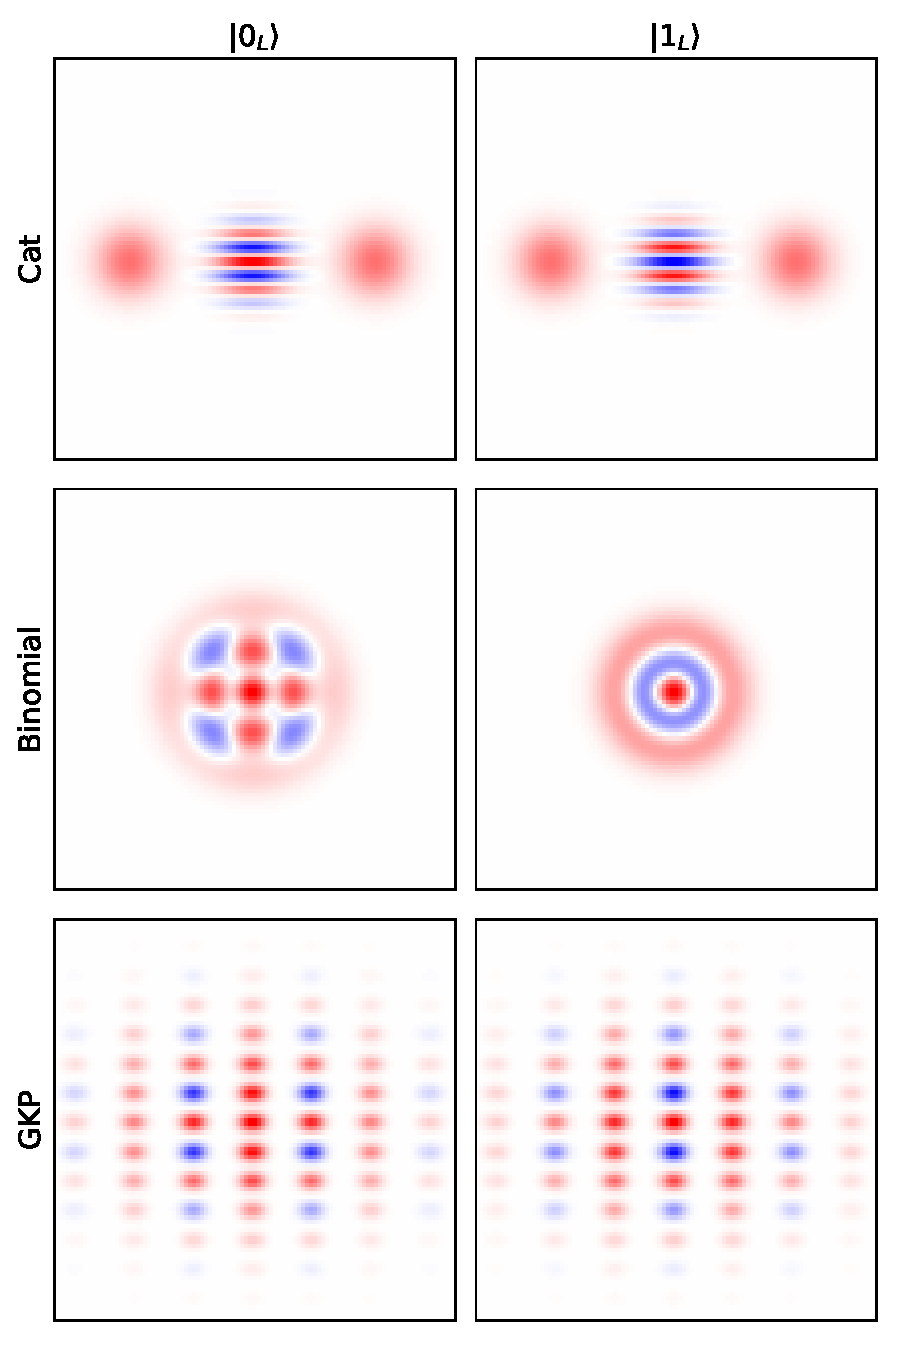
\includegraphics[width=0.8\columnwidth]{figures/cat_binom_gkp.pdf}
    \caption{Wigner functions for the logical qubit basis states in the cat, binomial, and GKP encodings.}
    \label{fig:cat_binom_gkp}
\end{figure}

Several bosonic encodings have been proposed.
For instance, binomial codes encode qubits as superpositions of Fock states, each of which is weighted by a binomial coefficient.
The lowest-order binomial code has logical basis states
\begin{align*}
    \ket{0_L} &= \left ( \ket{0} + \ket{4} \right ) / \sqrt{2}, \\
    \ket{1_L} &= \ket{2},
\end{align*}
and can protect against single-photon loss errors \cite{cai_2021,michael_2016}.
The Gottesman, Kitaev, and Preskill (GKP) code, on the other hand, defines the logical basis states as superpositions of squeezed states \cite{gottesman_2001}:
\begin{align*}
    \ket{0_L} &\propto \sum_{s=-\infty}^{\infty} \ket{q = 2 s \sqrt{\pi}}, \\
    \ket{1_L} &\propto \sum_{s=-\infty}^{\infty} \ket{q = (2 s + 1) \sqrt{\pi}}.
\end{align*}
The GKP code can protect against a variety of errors, but experimental implementation is difficult, and has only been demonstrated recently \cite{campagne_ibarcq_2020}.
See Cai et al. and Ma et al. \cite{cai_2021, ma_2021} for a review of recent progress in bosonic error correction codes.
Figure \ref{fig:cat_binom_gkp} shows the Wigner functions for these two encodings, as well as the cat code we consider for the remainder of this paper.

Perhaps the simplest bosonic code is the so-called cat code, which encodes logical qubits as superpositions of coherent states of an oscillator opposite to each other in phase, i.e. Schr\"odinger cat states \cite{cai_2021,mirrahimi_2014,puri_2017,ofek_2016,grimm_2020,ma_2021}.
These states are given by
\[
    \ket{\mathcal{C}_\alpha^\pm} = \mathcal{N}_\alpha^\pm \left ( \ket{\alpha} \pm \ket{-\alpha} \right )
\]
where the normalization is
\[
    \mathcal{N}_\alpha^\pm = \frac {1} {\sqrt{ 2 \left ( 1 \pm e^{-2\bar{n}} \right ) }}
\]
for average photon number $\bar{n} = |\alpha|^2$.
In its simplest form the logical basis states in this encoding are
\begin{align*}
    \ket{0_L} &= \ket{\mathcal{C}_\alpha^+}, \\
    \ket{1_L} &= \ket{\mathcal{C}_\alpha^-}.
\end{align*}
Note that these states have opposite photon number parity: $\ket{\mathcal{C}_\alpha^+}$ only includes Fock states of even photon number parity, while those for $\ket{\mathcal{C}_\alpha^+}$ are only odd.

The separation in phase space of these opposite-phase coherent states ensures that the quantum information is protected from small, local displacements in this phase space \cite{mirrahimi_2014,grimm_2020}.
Note in particular the effect of the photon annihilation operator $\hat{a}$ on the cat states:
\[
    \hat{a} \ket{\mathcal{C}_\alpha^\pm} = \ket{\mathcal{C}_\alpha^\mp};
\]
that is, the loss of a photon from the resonator induces a bit flip error, which might be detected through continuous measurements of photon number parity.
Such an error detection is not possible in this simple realization of a cat qubit, but it has been implemented for more complex variations \cite{ofek_2016}.
Despite the lack of a means of detecting and correcting errors, this encoding is nonetheless a useful resource for quantum computation.
It has been shown that the noise in this encoding is ``biased'': phase flip errors are suppressed exponentially in $\bar{n}$, while the bit flip rate only increases linearly in $\bar{n}$ \cite{puri_2017,puri_2019}.
When the noise is biased in this manner, additional layers of QEC can be focused on the dominant noise channel, i.e. bit flips.
Quantum logic gates that preserve this noise bias have been proposed, furthering the potential usefulness of this scheme \cite{puri_2020}.

The remainder of this paper is organized as follows: in Section \ref{sec:init} we discuss the initialization and stabilization of a cat qubit using a Kerr-nonlinear resonator and a two-photon squeezing drive.
In Section \ref{sec:gates} we discuss the implementation of single-qubit gates to drive rotations about the $X$ and $Z$ axes of the Bloch sphere.
In section \ref{sec:two_qubit} we extend the previous discussion of the operation of a single qubit to the case of two capacitively coupled Kerr-cat qubits.
For each aspect of the operation of these qubits we present numerical simulations using experimentally realistic parameters.

\section{\label{sec:init} Initialization and stabilization of a Kerr-cat qubit}

\begin{figure}[t]
    \centering
    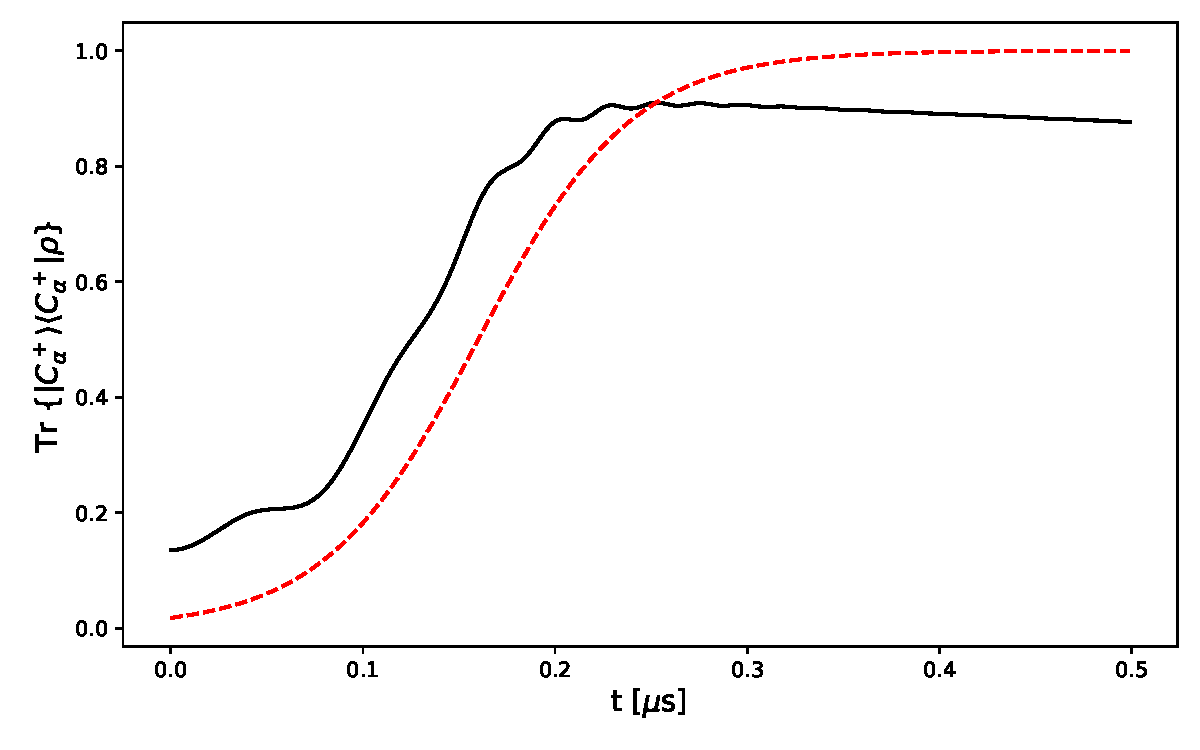
\includegraphics[width=\columnwidth]{figures/initialization.pdf}
    \caption{Initialization of the $\ket{\mathcal{C}_\alpha^+}$ cat state. The projection of the resonator state onto the target state is shown in black, while the squeezing drive envelope is shown in red.}
    \label{fig:initialization}
\end{figure}

\begin{figure}[t]
    \centering
    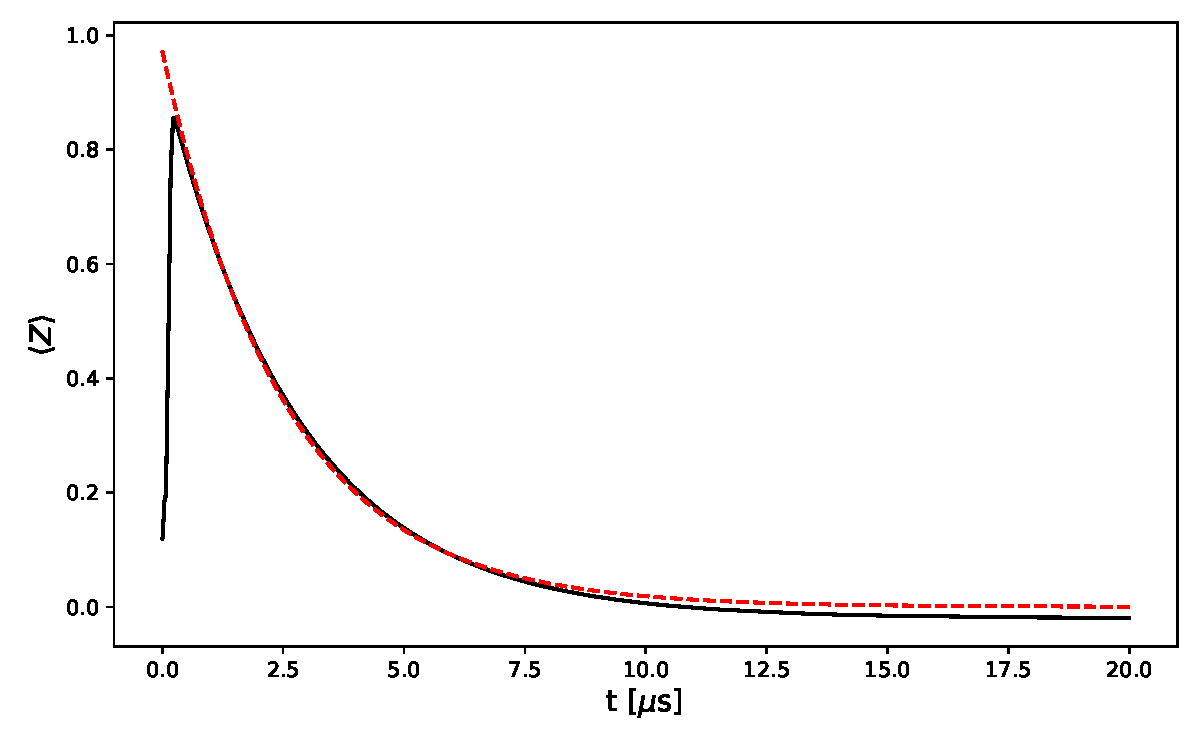
\includegraphics[width=\columnwidth]{figures/decay.pdf}
    \caption{Decay of the logical qubit due to decoherence. The red dashed line shows an exponential fit to the data after \SI{0.4}{\micro\s}, yielding a decay time of $\tau_Z =$ \SI{2.526}{\micro\s} $\pm$ \SI{0.002}{\micro\s}.}
    \label{fig:decay}
\end{figure}

\begin{figure*}[t]
     \centering
     \begin{subfigure}[b]{0.30\textwidth}
         \centering
         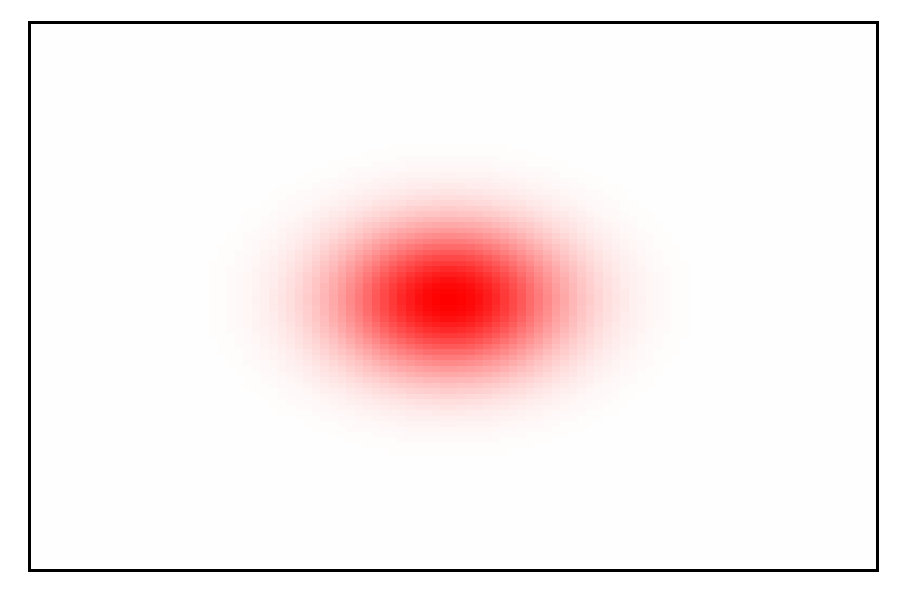
\includegraphics[width=\textwidth]{figures/ground.pdf}
         \caption{}
         \label{fig:ground}
     \end{subfigure}
     \hfill
     \begin{subfigure}[b]{0.30\textwidth}
         \centering
         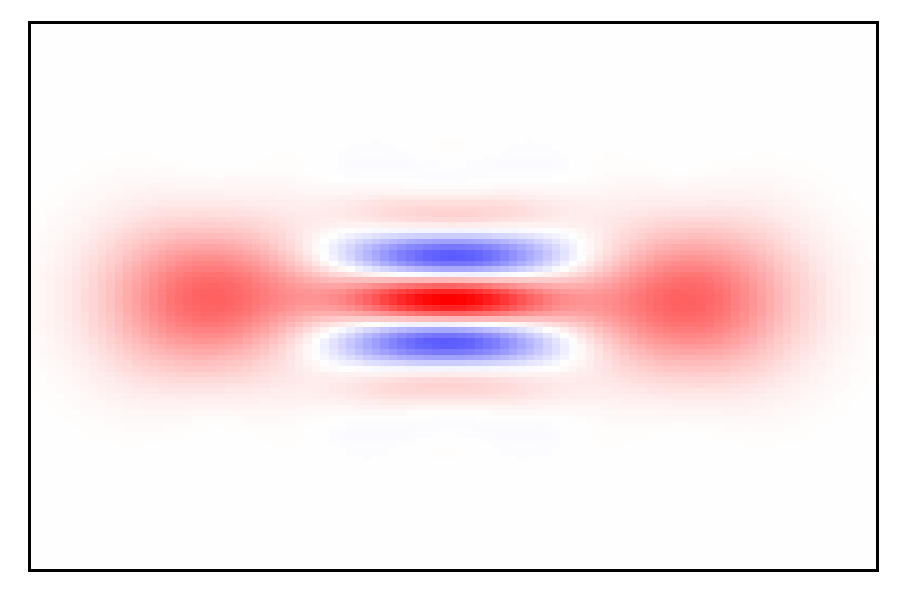
\includegraphics[width=\textwidth]{figures/initialized_cat.pdf}
         \caption{}
         \label{fig:initialized_cat}
     \end{subfigure}
     \hfill
     \begin{subfigure}[b]{0.30\textwidth}
         \centering
         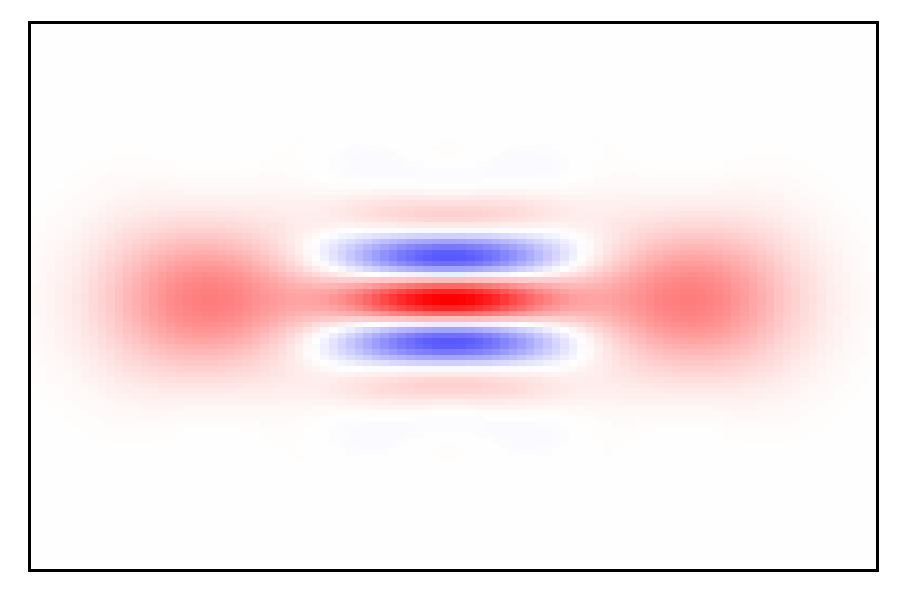
\includegraphics[width=\textwidth]{figures/ideal_cat.pdf}
         \caption{}
         \label{fig:ideal_cat}
     \end{subfigure}
        \caption{Wigner functions for (a) the initial thermal state, (b) the adiabatically initialized $\ket{0_L} = \ket{\mathcal{C}_\alpha^+}$ cat state, and (c) the ideal cat state.}
        \label{fig:initialization_wigner}
\end{figure*}

Cat states can be initialized and stabilized in a superconducting microwave resonator by introducing a Kerr nonlinearity and a two-photon squeezing drive, as proposed by Puri et al. and later realized experimentally by Grimm et al. \cite{puri_2017,grimm_2020}.
The experimental platform used by Grimm et al. consists of a nonlinear resonator placed within a 3D microwave cavity; the resulting nonlinearity facilitates the generation of a two-photon drive through three-wave mixing and is also responsible for the Kerr nonlinearity.
See \cite{grimm_2020}, particularly the supplementary information, for details.

The Hamiltonian describing this system in the absence of any other microwave drives (after a transformation to the frame rotating at the resonator frequency) is
\begin{equation}
    \hat{H}_{\rm sys} / \hbar = -K \hat{a}^{\dag 2} \hat{a}^2 + \epsilon_2 \hat{a}^{\dag 2} + \epsilon_2^* \hat{a}^2,
\end{equation}
where $K$ is the strength of the Kerr nonlinearity and $\epsilon_2$ is the two-photon drive strength.

This Hamiltonian has two degenerate lowest-energy eigenstates, specifically the coherent states $\ket{\pm \alpha}$ for $\alpha = \sqrt{\epsilon_2 / K}$.
Note that this Hamiltonian has the property of preserving photon number parity: photons are only created or destroyed two at a time.
In the absence of the two-photon drive, the lowest-energy eigenstate is simply the $\ket{0}$ Fock state, which has even photon number parity.
By ramping the squeezing drive on and off slowly with respect to $1/2K$, the $\ket{0}$ Fock state is adiabatically mapped onto the logical basis state $\ket{0_L} = \ket{\mathcal{C}_\alpha^+}$, due to the parity-preserving nature of the Hamiltonian.
This is the method demonstrated experimentally by Grimm et al. \cite{grimm_2020}.

Figure \ref{fig:initialization} shows a numerical simulation of this process.
The resonator is assumed to be initially in a thermal state with a population of $n_{\rm th} = 0.04$ in the $\ket{1}$ Fock state.
The strength of the Kerr nonlinearity is $K / 2\pi =$ \SI{6.7}{\MHz} and the two-photon drive is ramped up with a $\tanh$ pulse shape over a period of \SI{320}{\ns} to a final value of $\epsilon_2 / 2 \pi =$ \SI{15.5}{\MHz} (all system parameters are taken from Grimm et al. \cite{grimm_2020}).
The time evolution of the system is determined using the Lindblad master equation \cite{manzano_2020}:
\[
    \dot{\hat{\rho}} = - \frac {i} {\hbar} [\hat{H}_{\rm sys}, \hat{\rho}] + \kappa_a (1 + n_{\rm th}) \mathcal{D}[\hat{a}] \hat{\rho} + \kappa_a n_{\rm th} \mathcal{D}[\hat{a}^\dag] \hat{\rho}
\]
where $\kappa_a = 1/T_1$ is the single-photon loss rate (Grimm et al. measures $T_1 =$ \SI{15.5}{\micro\s} \cite{grimm_2020}) and
\[
    \mathcal{D}[\hat{\mathcal{O}}] \hat{\rho} = \hat{\mathcal{O}} \hat{\rho} \hat{\mathcal{O}}^\dag - \frac {1} {2} \hat{\mathcal{O}}^\dag \hat{\mathcal{O}} \hat{\rho} - \frac {1} {2} \hat{\rho} \hat{\mathcal{O}}^\dag \hat{\mathcal{O}}.
\]

Figure \ref{fig:initialization_wigner} shows the Wigner functions for the initial thermal state, adiabatically initialized cat state, and the ideal cat state, demonstrating the effectiveness of the adiabatic mapping in initializing the cat qubit.
The imperfect initialization (visible in Figure \ref{fig:initialization}) is primarily due to the nonzero population of the $\ket{1}$ Fock state in the resonator's initial thermal state and photon loss in the resonator.

Figure \ref{fig:decay} shows the decay of the qubit's $\langle Z \rangle$-component when initialized to the $\ket{\mathcal{C}_\alpha^+}$ state.
An exponential fit to this curve yields a decay time of $\tau_Z =$ \SI{2.526}{\micro\s} $\pm$ \SI{0.002}{\micro\s}; this is close to, albeit just outside the uncertainty of, the experimentally measured value of $\tau_Z =$ \SI{2.60}{\micro\s} $\pm$ \SI{0.07}{\micro\s} reported by Grimm et al. \cite{grimm_2020}.

\section{\label{sec:gates} Single-qubit gate operations}

Having characterized the initialization and subsequent decoherence of a Kerr-cat qubit, we now turn our attention to universal single-qubit control, realized in an $X(\theta)$ gate for arbitrary $\theta$ and a $Z(\pi/2)$ gate.
In particular, we wish to show that these gates can be performed in a time much shorter than the qubit's decoherence time.

\subsection{Arbitrary $X$ rotations}

One can show that the application of an additional coherent drive induces Rabi oscillations in the encoded qubit: in particular, the Hamiltonian
\begin{equation} \label{eq:x}
    \hat{H}_x / \hbar = \epsilon_x \hat{a}^\dag + \epsilon_x^* \hat{a},
\end{equation}
when projected onto the subspace spanned by $\{ \ket{\mathcal{C}_\alpha^+}, \ket{\mathcal{C}_\alpha^-}\}$, has the form \cite{grimm_2020,mirrahimi_2014}
\[
    \Omega_x \sigma_x^L
\]
where the superscript $L$ indicates that we are working in the logical qubit basis and
\[
    \Omega_x = {\rm Re}(2 \epsilon_x \sqrt{\bar{n}}).
\]
Evolution of the cat qubit under this Hamiltonian has the effect of inducing Rabi oscillations, much like a two-level system under the same coherent drive.
One can gain some intuition for this interaction by considering the effect of Eq. (\ref{eq:x}) on the photon number parity: the exchange of single photons caused by this drive has the effect of swapping photon number parity, corresponding to transitions between $\ket{\mathcal{C}_\alpha^+}$ and $\ket{\mathcal{C}_\alpha^-}$.

In Figure \ref{fig:rabi} we show the time evolution of the cat qubit using a relatively low drive strength of $\epsilon_x / 2 \pi =$ \SI{170}{\kHz}.
The qubit is clearly undergoing Rabi oscillations.
Note, however, that these Rabi oscillations differ from those of a two-level system in an important way: the oscillation frequency varies with the amplitude and phase of the drive.
When using this effect to implement the $X(\theta)$ gate, we can therefore choose a large drive amplitude to make the gate time very short.
Evolution of the cat qubit under the coherent drive for a time $t_x = \theta / 2 \Omega_x$ effects an $X(\theta)$ gate on the qubit; this gate is demonstrated in Figure \ref{fig:x_gate} for a rotation by $\theta = \pi$ using a drive strength of $\epsilon_x / 2 \pi =$ \SI{6}{\MHz}.

\begin{figure}[t]
    \centering
    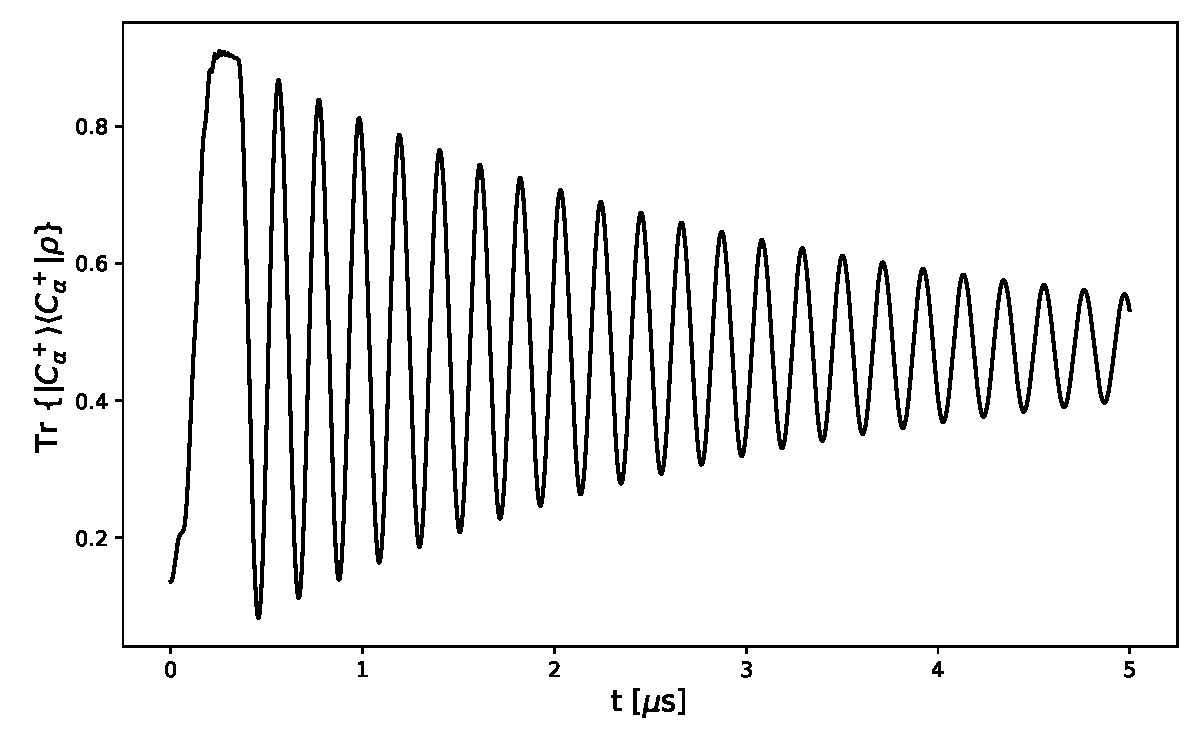
\includegraphics[width=\columnwidth]{figures/rabi.pdf}
    \caption{Rabi oscillations driven by a coherent resonant drive.}
    \label{fig:rabi}
\end{figure}

\subsection{The $Z(\pi/2)$ gate}

Having implemented rotations by an arbitrary angle about the $X$-axis of the cat-qubit's Bloch sphere, all that is needed to reach any point on the sphere is a $\pi/2$ rotation about the $Z$-axis.
This gate is realized as the evolution of the cat-qubit under the Kerr Hamiltonian in the absence of any drives.
In particular, this evolution for a time $t_z = \pi/2K$ maps the coherent states $\ket{\pm \alpha}$ onto $(\ket{\pm \alpha} - i \ket{\mp \alpha}) / \sqrt{2}$, thus inducing a rotation by $\pi/2$ about the $Z$-axis of the Bloch sphere \cite{grimm_2020,mirrahimi_2014}.

Figure \ref{fig:bloch} shows the projection of the resonator state onto the Bloch states $\ket{\pm X}$, $\ket{\pm Y}$, and $\ket{\pm Z}$ under the application of an $X(\pi/2)$ gate followed by a $Z(\pi/2)$ gate.
We see that the qubit is first initialized in the $\ket{+Z} = \ket{\mathcal{C}_\alpha^+}$ state, then rotated about the $X$-axis onto the $\ket{-Y} = (\ket{\mathcal{C}_\alpha^+} - i \ket{\mathcal{C}_\alpha^-}) / \sqrt{2}$ state.
Following this it is rotated by $\pi/2$ about the $Z$-axis onto the $\ket{+X} = (\ket{\mathcal{C}_\alpha^+} + \ket{\mathcal{C}_\alpha^-}) / \sqrt{2}$ state, as we would expect.
Through sequences of $X(\theta)$ and $Z(\pi/2)$ gates we could in principle reach any point on the Bloch sphere.

\begin{figure}[t]
    \centering
    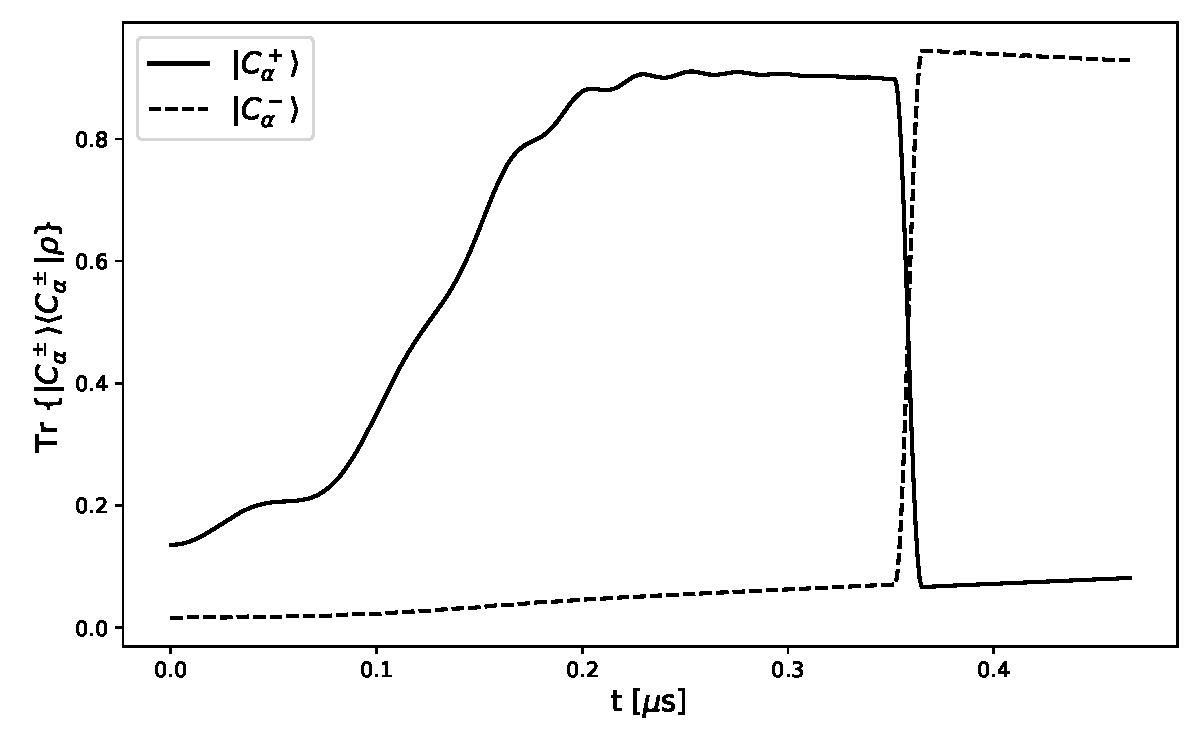
\includegraphics[width=\columnwidth]{figures/x_gate.pdf}
    \caption{Bit flip due to the application of an $X(\pi)$ gate.}
    \label{fig:x_gate}
\end{figure}


\begin{figure}[t]
    \centering
    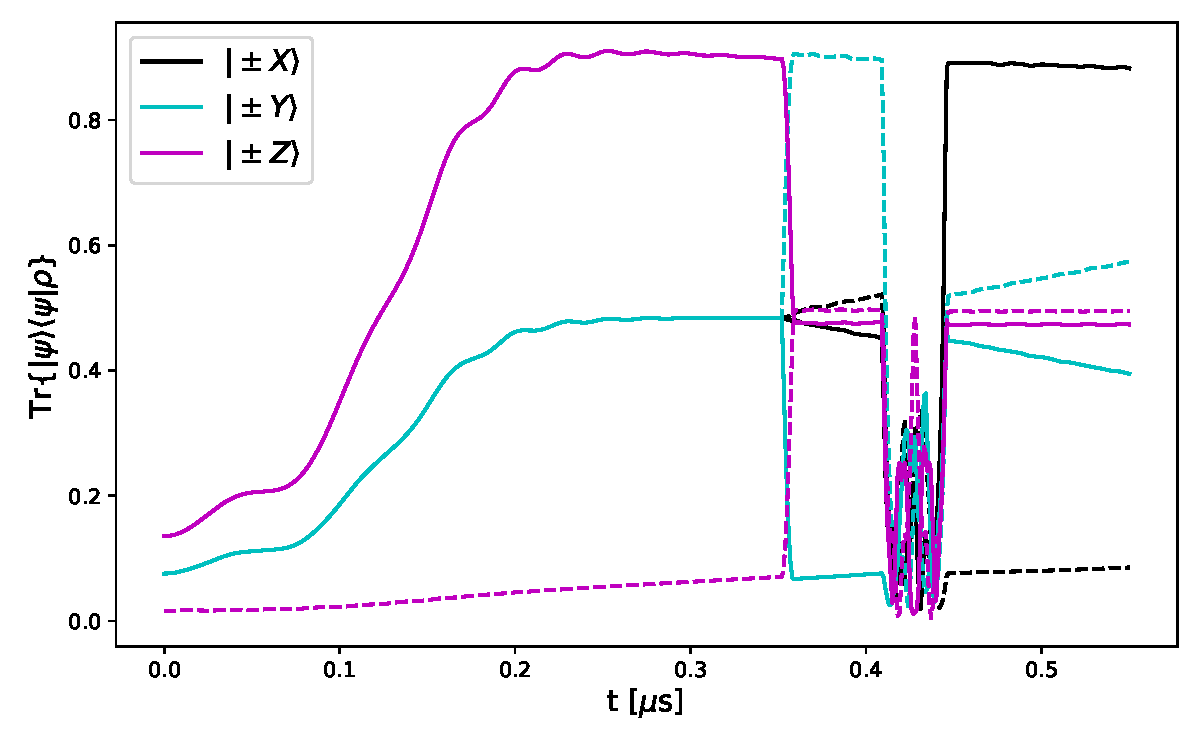
\includegraphics[width=\columnwidth]{figures/bloch.pdf}
    \caption{Projection of the cat-qubit state onto the states corresponding to the axes of the Bloch sphere during state initialization and the application of an $X(\pi/2)$ gate followed by a $Z(\pi/2)$ gate. Solid lines correspond to the positive direction on the Bloch sphere axis while dashed lines correspond to the negative direction.}
    \label{fig:bloch}
\end{figure}

\section{\label{sec:two_qubit} The two-qubit entangling gate}

While Grimm et al. \cite{grimm_2020} is concerned principally with the stabilization and operation of a single qubit, one can imagine capacitively coupling two of these resonators, resulting in the coupling Hamiltonian
\begin{equation}
    \hat{H}_c / \hbar = \chi(t) (\hat{a}_1^\dag \otimes \hat{a}_2 + \hat{a}_1 \otimes \hat{a}_2^\dag)
\end{equation}
where $\chi(t)$ is the coupling strength and the operator subscripts denote the subsystem on which the operator acts.
For simplicity we assume the coupling can be turned on and off, which might be realized experimentally by bringing the qubits in and out of resonance with one another or through some more complex coupling scheme \cite{wendin_2017}.
We further assume that both resonators have identical physical parameters.
We now have a four-dimensional logical qubit basis spanned by the states $\ket{\mathcal{C}_\alpha^\pm} \otimes \ket{\mathcal{C}_\alpha^\pm}$, which for notational simplicity will henceforth be denoted $\{\ket{00}, \ket{01}, \ket{10}, \ket{11}  \}$ (not to be confused with Fock states).

\begin{figure}[t]
    \centering
    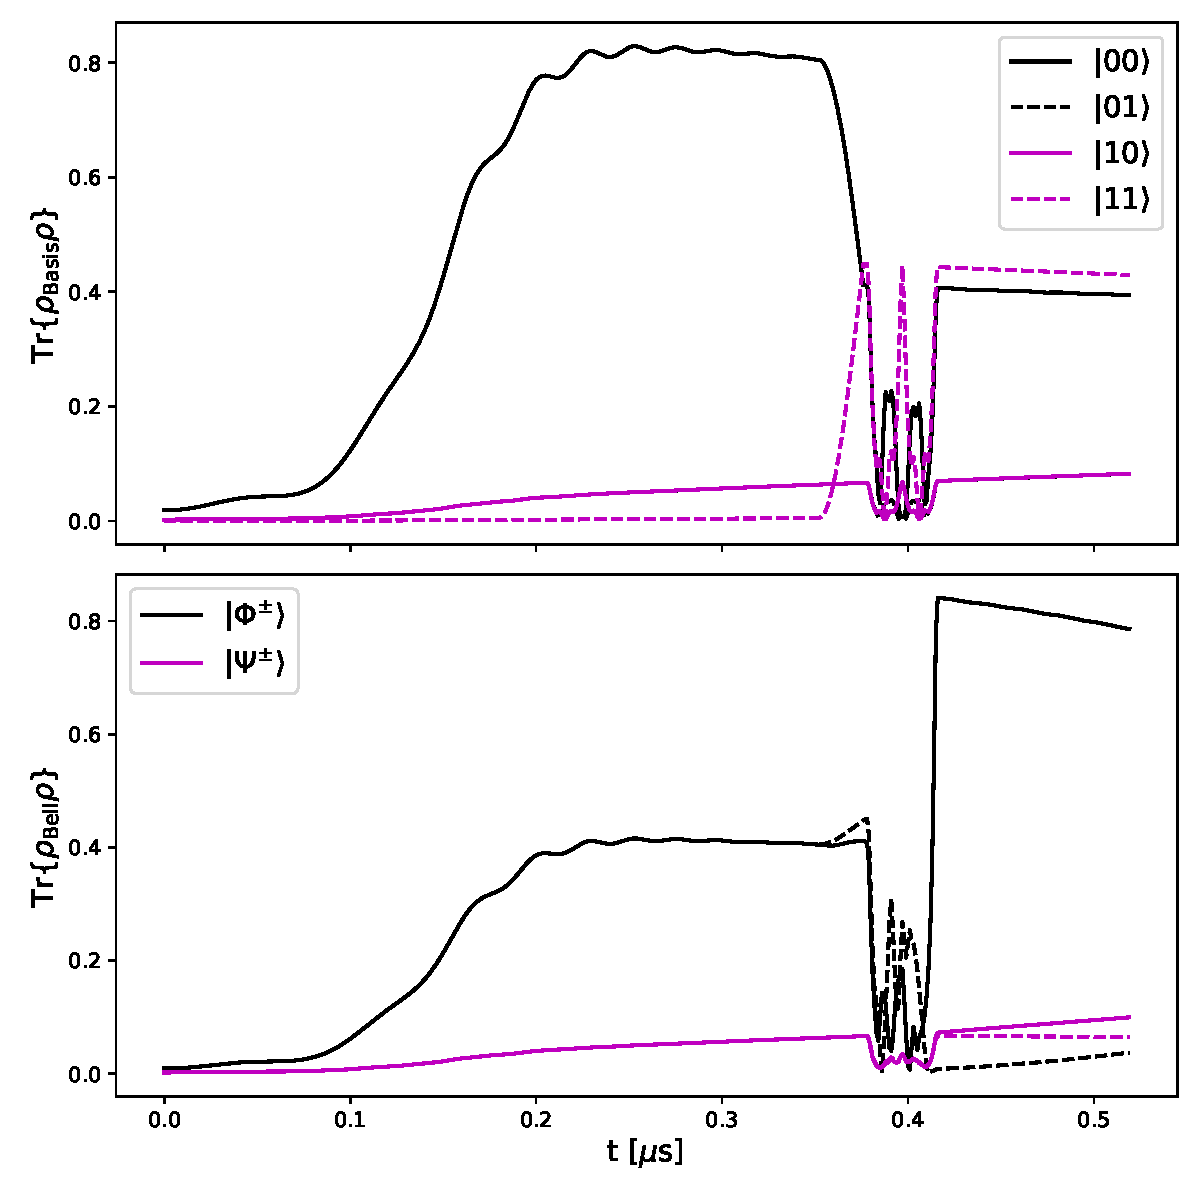
\includegraphics[width=\columnwidth]{figures/bell.pdf}
    \caption{Bell state generation gate sequence. We plot both the projection of the two-qubit state onto each of the logical basis states (upper) and the projection onto the Bell states (lower).}
    \label{fig:bell}
\end{figure}


\begin{figure*}[t]
     \centering
     \begin{subfigure}[b]{0.31\textwidth}
         \centering
         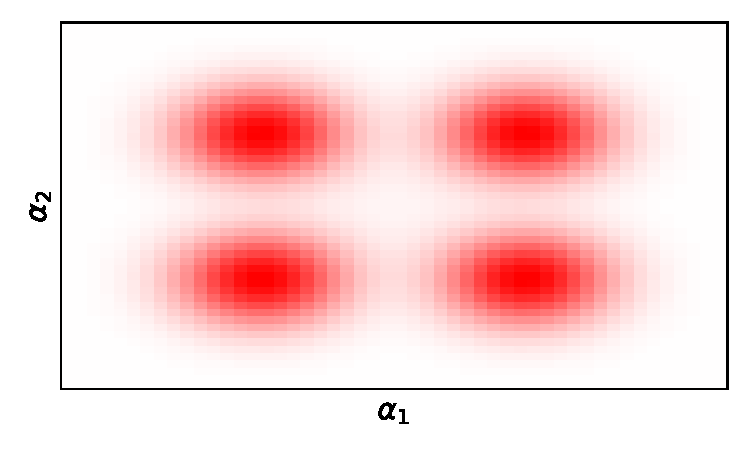
\includegraphics[width=\textwidth]{figures/q_mixed.pdf}
         \caption{}
         \label{fig:ground}
     \end{subfigure}
     \hfill
     \begin{subfigure}[b]{0.31\textwidth}
         \centering
         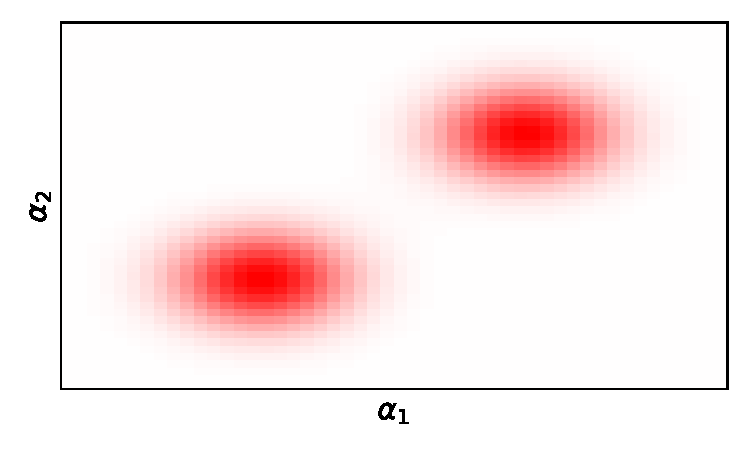
\includegraphics[width=\textwidth]{figures/q_entangled.pdf}
         \caption{}
         \label{fig:initialized_cat}
     \end{subfigure}
     \hfill
     \begin{subfigure}[b]{0.31\textwidth}
         \centering
         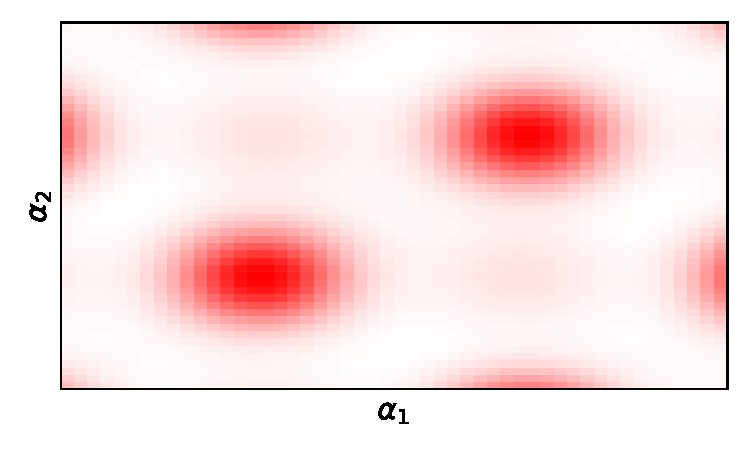
\includegraphics[width=\textwidth]{figures/q_actual.pdf}
         \caption{}
         \label{fig:ideal_cat}
     \end{subfigure}
        \caption{Husimi $Q$ functions for (a) a mixed state, (b) an ideal entangled state, and (c) the result of applying the entangling gate followed by a $Z(\pi/2)$ gate. The Husimi $Q$ function is in reality a function of two complex numbers, but here we show a two-dimensional representation restricted to real values of $\alpha_1$ and $\alpha_2$. The secondary peaks visible on the result of the simulation (c) are an artifact of the finite-dimensional Hilbert space ($n=0,\ldots,10$ for each resonator). Running the simulation in a higher-dimensional Hilbert space would remove these, but the increased computational cost makes this infeasible.}
        \label{fig:Q}
\end{figure*}

When projected onto the subspace spanned by this basis, the coupling Hamiltonian takes the form \cite{mirrahimi_2014}
\[
    \Omega_c \sigma_{x,1}^L \otimes \sigma_{x,2}^L
\]
where
\[
    \Omega_c = 2 \bar{n} \chi(t).
\]
Evolution of the two-qubit system under this Hamiltonian for a time $t_c = \pi/4\Omega_c$ has the effect of entangling the cat-qubits: this entangling gate can be expressed as the unitary operation
\[
    E^L = \frac {1} {\sqrt{2}} \begin{bmatrix}
        1 & 0 & 0 & -i \\
        0 & 1 & -i & 0 \\
        0 & -i & 1 & 0 \\
        -i & 0 & 0 & 1
    \end{bmatrix},
\]
which acts on the logical (encoded) qubit rather than the resonator Fock states.

By composing this two-qubit entangling gate with $X$ and $Z$ gates applied to individual qubits we can create Bell states in the logical qubit space.
For example, Figure \ref{fig:bell} demonstrates the creation of a $\ket{\Phi^+}$ Bell state by applying the entangling gate to the two-qubit system followed by applying a $Z(\pi/2)$ gate to the first qubit.
This is represented in both the logical qubit basis and the Bell state basis.

In addition to plotting the projection of the two-qubit state onto the target Bell state, as in Figure \ref{fig:bell}, we can also attempt to confirm the presence of entanglement by visualizing the phase space of the two-qubit system.
Because the Wigner function for a bipartite system is difficult to compute, we instead compute the Husimi $Q$ function, defined in the case of a bipartite system as
\begin{equation} \label{eq:Q}
    Q(\alpha_1, \alpha_2) = \bra{\alpha_1} \otimes \bra{\alpha_2} \hat{\rho} \ket{\alpha_1} \otimes \ket{\alpha_2}.
\end{equation}
In principle this is a quasiprobability distribution over four real numbers, since $\alpha_1$ and $\alpha_2$ are complex.
For simplicity and ease of plotting we take $\alpha_1, \alpha_2 \in \mathbb{R}$.

For a separable state, i.e. $\hat{\rho} = \hat{\rho}_1 \otimes \hat{\rho}_2$, the $Q$ function factorizes \cite{floerchinger_2022}:
\[
    Q(\alpha_1, \alpha_2) = Q_1(\alpha_1) Q_2(\alpha_2).
\]
Suppose the $Q$ function for such a separable state in our two-dimensional representation has peaks at $(\alpha_1, \alpha_2)$ and $(-\alpha_1, -\alpha_2)$.
The above factorization implies that the $Q$ function must have peaks at $(-\alpha_1, \alpha_2)$ and $(\alpha_1, -\alpha_2)$ as well, while this need not be the case for a non-separable (i.e. entangled) state.
Finally, note that by Eq. (\ref{eq:Q}) the $Q$ function of a statistical mixture is the sum of the $Q$ functions of its constituent parts.

Figure \ref{fig:Q} shows the $Q$ functions for the statistical mixture $\hat{\rho} = (\ket{00}\bra{00} + \ket{11}\bra{11}) / 2$, the entangled state $\ket{\Phi^+} = (\ket{00} + \ket{11}) / \sqrt{2}$ in the ideal case, and the same entangled state as generated in the numerical simulation.
Note that the statistical mixture and the entangled state both have the same measurement probabilities in the logical qubit basis, and are therefore indistinguishable when only considering such measurements.
The $Q$ functions, however, demonstrate the presence of bipartite entanglement: the statistical mixture obeys the above requirement regarding the locations of its peaks, while the entangled state does not.
Because $Q$ functions are experimentally accessible \cite{kirchmair_2013,floerchinger_2022}, measurements of it could possibly be used to confirm the presence of entanglement in an experimental implementation of the coupling described here.

\section{Conclusion}

Schr\"odinger cat states, i.e. quantum superpositions of coherent states, present a compelling opportunity for the implementation of error-protected qubits.
In particular, these cat states can be created in a superconducting microwave resonator with a Kerr nonlinearity and subsequently used as the logical qubit basis states in a quantum error correction scheme.
Individual cat-qubits can be adiabatically initialized and subsequently stabilized by applying a two-photon squeezing drive, as demonstrated by Grimm et al. \cite{grimm_2020}.
Furthermore, universal control of these qubits is straightforward, requiring only the application of a coherent microwave drive or the turning off of the squeezing drive.

An obvious extension to the operation of this Kerr-cat qubit is to capacitively couple two of them together, as proposed by e.g. Mirrahimi et al. \cite{mirrahimi_2014}.
Under this capacitive coupling the two-qubit system becomes entangled, allowing for the initialization and control of arbitrary two-qubit states.

In this paper we have numerically simulated the initialization and operation of single- and two-qubit systems composed of Kerr-cat qubits, using the experimentally measured system parameters determined by Grimm et al. \cite{grimm_2020} where possible.
Using these simulations we have replicated some of the experimental results, including the operation of single-qubit gates.
We have also simulated the evolution of the system under the capacitive coupling Hamiltonian and demonstrated that it can entangle the qubits in a time far shorter than these qubits' decoherence times.
Finally, we have demonstrated that measurements of the two-qubit $Q$ function could in principle be used to distinguish between bipartite entanglement and statistical mixtures, though more work is needed to confirm that this is experimentally feasible for the particular system at hand.



\bibliography{citations}

\end{document}
